\subsection{Модуль хранения истории} \label{research_history}

Одной из важных функций системы электронного документооборота и КХЭД как её части является хранение истории внесённых изменений. Это необходимо не только для учёта затраченного времени, но и для разбора конфликтных ситуаций, а также возможности создавать несколько документов на базе одного. Необходимость хранения полной и достоверной истории изменения документа описана в ГОСТ Р ИСО 15489-1 --- 2007 (см. главу \ref{rights_gost_15489_1}). Однако, как показало исследование \ref{review_products}, компании-разработчики СЭД не афишируют способы организации хранения истории, полностью полагаясь на средства СУБД в вопросе обеспечения целостности данных.

\vspace{\baselineskip}
В общем случае, при таком подходе каждая запись в истории хранится в виде автономного объекта, к которому необходимо добавлять метку времени для упорядочивания событий во временн\textit{о}м порядке, а также электронную подпись для установления авторства.

\vspace{\baselineskip}
В качестве альтернативы предлагается другой способ хранения истории изменений --- в виде цепочки хэш-сумм, как показано на рис. \ref{img:git_hash}. В такой структуре каждая запись содержит в себе контрольную сумму (хэш-сумму) предыдущей записи. Таким образом, события связываются в порядке появления, что избавляет от необходимости дополнительно устанавливать отношения между ними. Дополнительным преимуществом такой схемы является сложность её подделки: если в случае атомарных записей злоумышленник атакует одну целевую запись, то в случае цепочки помимо атаки на целевую запись необходимо также подделать все записи, появившиеся после неё, чтобы целостность цепи не была нарушена. Сложность такой атаки возрастает с увеличением длины цепи.
\begin{figure}[h!]
  \centering
  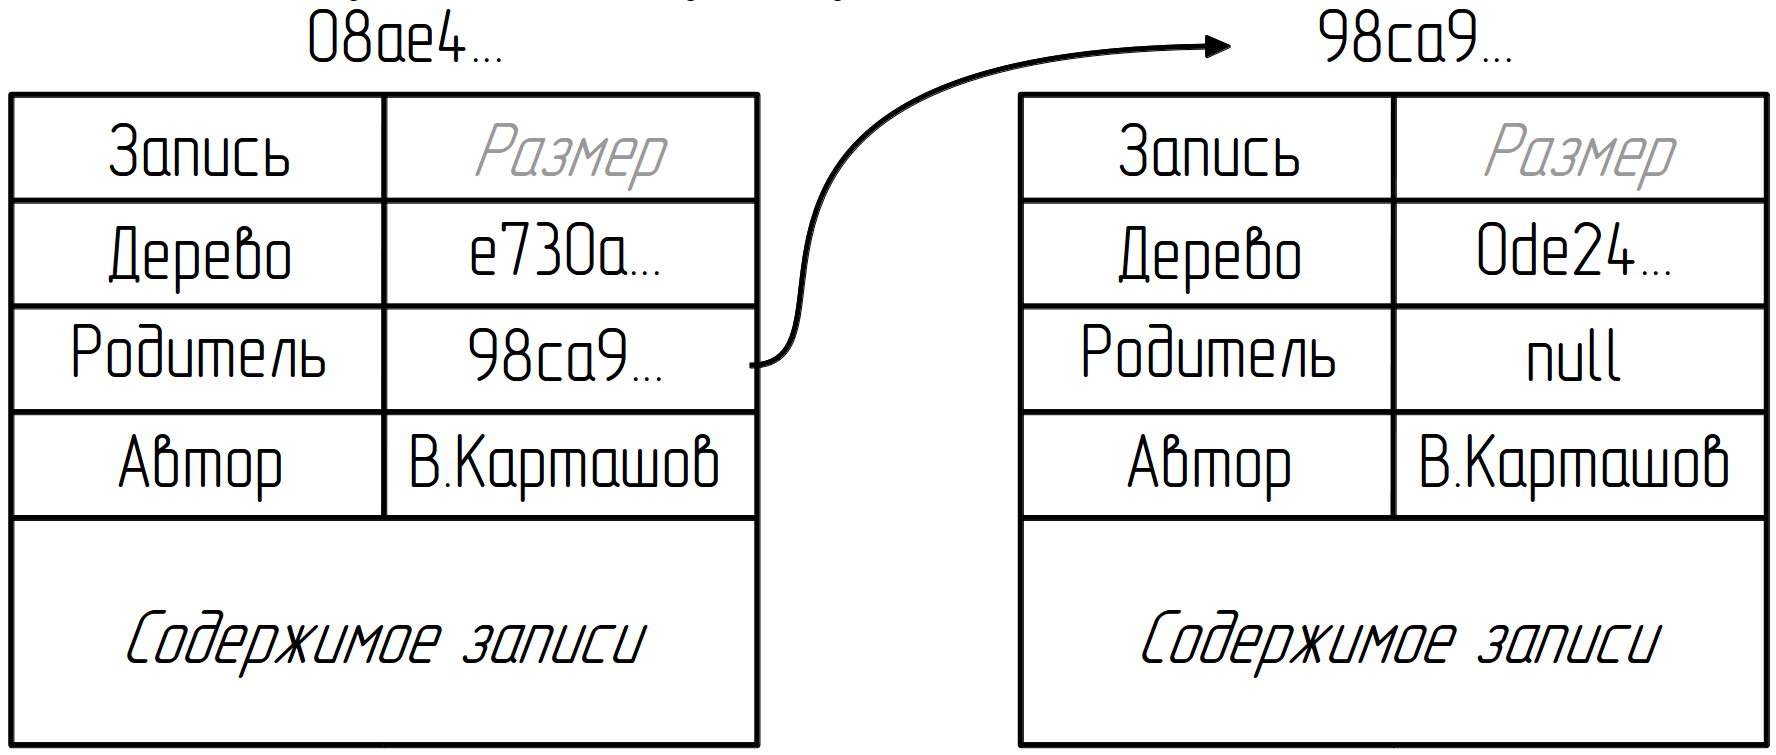
\includegraphics[width=1\textwidth]{git_hash}
  \caption{Общий вид цепочки хэш-сумм}
  \label{img:git_hash}
\end{figure}

\vspace{\baselineskip}
В случае дополнения каждой записи электронной подписью становится возможным просматривать документ с построчным указанием авторства, как показано на рис. \ref{img:git_blame}.

\begin{figure}[h!]
  \centering
  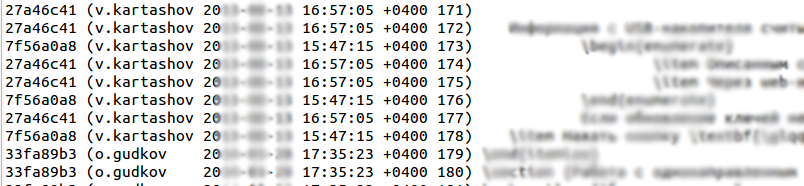
\includegraphics[width=1\textwidth]{git_blame}
  \caption{Просмотр документа с построчным указанием авторства}
  \label{img:git_blame}
\end{figure}

\vspace{\baselineskip}
Таким образом, для проверки целостности истории в первом случае необходимо проверить метку времени каждой записи, а во втором --- лишь убедиться в совпадении соответствующих хэш-сумм. Если последняя операция может считаться атомарной в соответствии с ГОСТ Р 34.11, то проверка метки времени состоит как минимум из трёх операций: сверки хэш-суммы, проверки электронной подписи сервера доверенного времени и проверки электронной подписи удостоверяющего центра, выдавшего сертификат серверу доверенного времени.

\vspace{\baselineskip}
Однако, замеры реализации данных функций средствами openssl не показали большой разницы в результатах: $0.03$ сек. для подсчёта контрольной суммы и $0.05$ сек. для проверки метки времени того же объекта. Это можно объяснить тем, что все операции, необходимые для проверки метки времени, являются независимыми и могут выполняться параллельно.

\vspace{\baselineskip}
Для проверки целостности истории, содержащей 800 записей, в соответствии с описанными замерами была построена схема для имитационного моделирования. Результаты временных замеров представлены на рис. \ref{img:historycheck_time}.

\begin{figure}[h!]
  \centering
  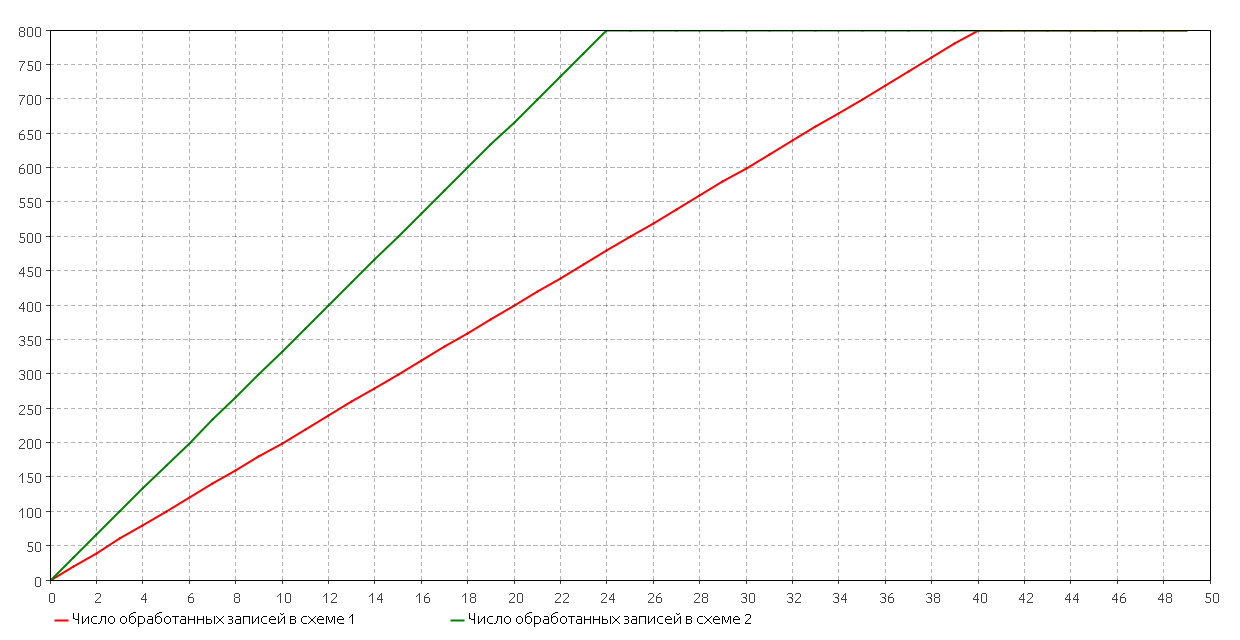
\includegraphics[width=1\textwidth]{historycheck_time}
  \caption{Время проверки целостности истории из 800 записей}
  \label{img:historycheck_time}
\end{figure}

\vspace{\baselineskip}
Как показал эксперимент, даже при таком большом объёме данных и несмотря на то, что система с использованием цепочки хэш-сумм сработала быстрее в $1,7$ раз, разница в реальном времени составила всего 16 секунд, что для конечного пользователя может быть не существенно. Однако описанный метод имеет другие достоинства: возрастающая с увеличением длины цепочки сложность подделки записей, отсутствие необходимости в содержании сервера доверенного времени. Это позволяет говорить о целесообразности применения такого метода для хранения полной и достоверной истории сделанных изменений.